\subsection{Derivation of Cable OBF}\label{sec:signal_representation}
To construct a detector, we decompose the signal into orthonormal components, \(S(\tau)\) can be written as \(S(\tau) = \sum_{n=1}^{2} a_n\, f_n(\tau).\)
where \(f_n(\tau\)) are the only terms that depend on time.
\begin{equation*}
    S(\tau) = \underbrace{K_p \cdot\cos\psi \cdot \cos\delta }_{{a_1}}                
              \underbrace{\frac{1}{1+\tau^2}}_{{f_1(\tau)}}
              +
              \underbrace{K_p \cdot\sin\delta}_{{a_2}}              
              \underbrace{\frac{\tau}{1+\tau^2}}_{{f_2(\tau)}}
\end{equation*}

Similar to the Anderson functions for dipoles, we can propose \(f_1(\tau)\) and \(f_2(\tau)\) as basis functions for cables, they just need to be orthonormalized, satisfying the following criteria:

\begin{equation*}
    \int_{-\infty}^{+\infty} \Phi_i(\tau)\, \Phi_j(\tau)\, d\tau = \delta_{ij}
\end{equation*}

where $\delta_{ij}$ is the Kronecker delta:

\[
    \delta_{ij} =
    \begin{cases}
        1 & \text{if } i = j \\
        0 & \text{if } i \neq j
    \end{cases}
\]
As the functions are already orthogonal, it is sufficient to normalize them, thus, we assume:
\begin{equation*}
    \Phi_1 = \kappa_1 f_1, \qquad \Phi_2 = \kappa_2 f_2
\end{equation*}
Solving for the normalization constants yields:

\begin{equation*}
    \kappa_1 = \kappa_2 = \sqrt{\frac{2}{\pi}}
\end{equation*}

The orthonormal basis functions for a cable carrying a DC current are therefore given by
\begin{equation}
    \Phi_1(\tau) = \sqrt{\frac{2}{\pi}}\,\frac{1}{1+\tau^2}, \qquad
    \Phi_2(\tau) = \sqrt{\frac{2}{\pi}}\,\frac{\tau}{1+\tau^2},
    \label{eq:OBF}
\end{equation}
where the normalized time parameter is defined as \(\tau = \frac{v\sin\theta}{d}\,t\).

\highlight{These OBF are plotted in Figure~\ref{fig:basis_funs} alongside MOBF from \cite{chenevas2025multipolar}, for order 1, which are the well-known Anderson functions for dipoles, and order 2, which combines the basis functions of a dipole and a quadrupole.}

Finally substituting equation~\eqref{eq:OBF} into the expression for the magnetic anomaly in equation~\ref{eq:anomaly},
yields the final anomaly signal representation for detection:
\begin{equation}
    S(\tau) = A_1\Phi_1(\tau) + A_2\Phi_2(\tau),
    \label{eq:anomaly_final}
\end{equation}
where \(A_1\) and \(A_2\) are the OBF amplitudes determined by the current, cable depth and orientation.

\begin{figure*}[t]
    \centering
    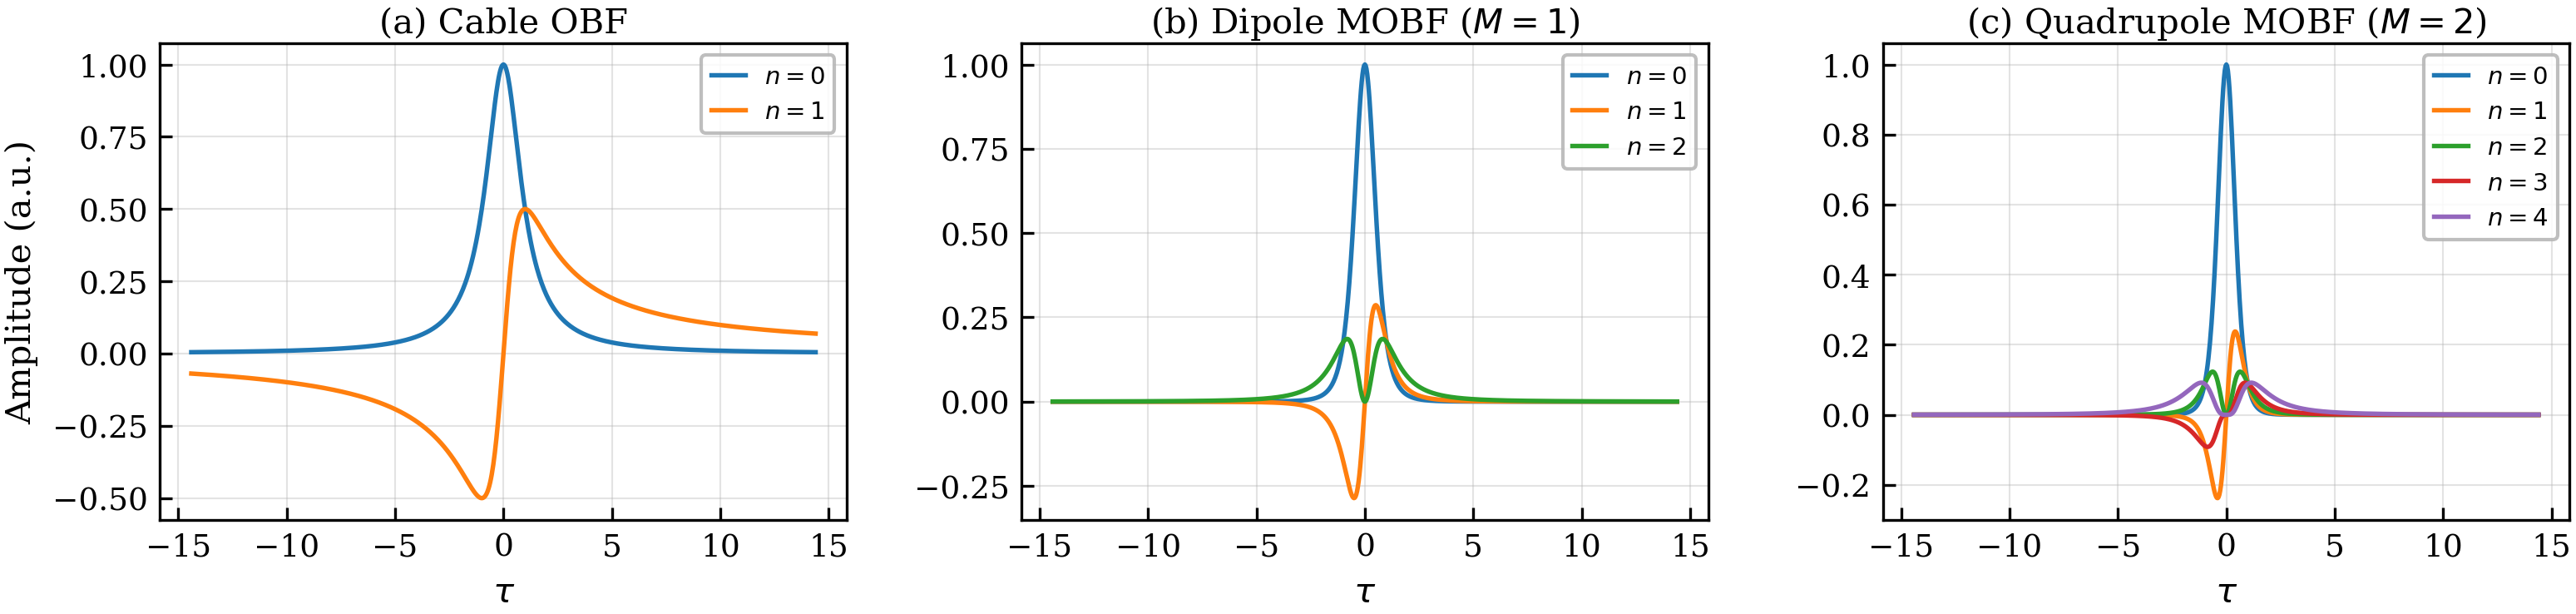
\includegraphics[width=\textwidth]{results_and_discus/figures/basis_functions_multipole.png}
    \caption{Basis functions for dipole and cable.}
    \label{fig:basis_funs}
\end{figure*}
